\begin{frame}
	\frametitle{SAT}
\vspace{-0.5cm}
  \begin{itemize}
    \item SAT formula in CNF
    $$\mathcal{F} = (x_1 \lor x_2 \lor \overline{x_3}) \land (x_3 \lor x_4)$$
    \vspace{-0.5cm}
    	\begin{itemize}
    		\item Boolean variables $x_1, x_2, \ldots, x_n$
    		\item Negations $\overline{x_1}, \ldots, \overline{x_n}$
    		\item Clauses: Disjunction of variables and their negations
    		\item $\mathcal{F}$: Conjuction of clauses
    	\end{itemize}
    %\item local functions $\cong$ clauses
    \item Is there an assignmnent of the variables that satisfies $\mathcal{F}$?
    \item How does the assignment look like?
  \end{itemize}
\end{frame}

\begin{frame}
	\frametitle{Factor Graphs}
	\vspace{-0.5cm}
		Factor graphs represent a function's factorization
		
		\begin{itemize}
			\item Function $f(X)$ over variables $X = \{x_1, x_2, \ldots, x_n\}$
			\item Global function $f$ factorizes to local functions
			$$ f(X) = \prod_{j=1}^m f_j(S_j)$$
			\item Local functions have smaller input $S_j \subset X$
		\end{itemize}
\end{frame}

\begin{frame}
	\frametitle{Factor Graphs}
		Factor graphs represent a function's factorization
		
		\begin{itemize}
			\item Two types of nodes
				\begin{itemize}
					\item Variable nodes: represent variables
					\item Factor nodes  : represent local functions
				\end{itemize}
			\item Edges connect variable and factor nodes
			\item Factor nodes are connected to all variable nodes of their input variables
		\end{itemize}
\end{frame}


\begin{frame}
	\frametitle{Example}
		\begin{align*}
		f(x_1, x_2, x_3) &= x_1^3 - x_1^2x_2 + x_1^2x_3 - x_1x_2x_3 \\
		&= \underbrace{(x_1)}_{f_1(x_1)} \cdot \underbrace{(x_1 - x_2)}_{f_2(x_1, x_2)} \cdot \underbrace{(x_1 + x_3)}_{f_3(x_1, x_2)}
\end{align*}		 

\begin{figure}
\centering

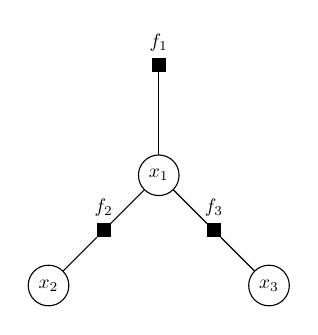
\begin{tikzpicture}[scale=0.7,transform shape]
   	\node[shape=circle,draw=black] (x1) at (0,0) {$x_1$};
    \node[shape=circle,draw=black] (x2) at (-2,-2) {$x_2$};
    \node[shape=circle,draw=black] (x3) at (2,-2) {$x_3$};
    \node[rectangle,draw=black, label = {$f_1$}, fill] (f1) at (0,2) {};
    \node[rectangle, fill, draw=black, label = {$f_2$}] (f2) at (-1,-1) {};
    \node[rectangle, fill, draw=black, label = {$f_3$}] (f3) at (1, -1) {} ;

    \path [-] (x1) edge node[left] {} (f1);
    \path [-] (x1) edge node[left] {} (f2);
    \path [-] (x1) edge node[left] {} (f3);
    \path [-] (f2) edge node[left] {} (x2);
    \path [-] (f3) edge node[left] {} (x3);
   
\end{tikzpicture}


\end{figure}
\end{frame}



\begin{frame}
	\frametitle{Factor Graphs}
	Factor Graph of a CNF formula
\begin{minipage}[0.2\textwidth]{\textwidth}
\begin{columns}[T]
\begin{column}{0.5\textwidth}
		
		\begin{align*}
			\mathcal{F} \;= \;&(x_1 \lor x_2 \lor {x_3}) \land (\overline{x_1} \lor x_2 \lor x_4) \\ & \land (\overline{x_3} \lor x_4) \land (\overline{x_1} \lor \overline{x_2})
		\end{align*}
		\begin{itemize}
			\item $\mathcal{F}$ is a product of clauses
			\item Clauses $\cong$ local functions
		\end{itemize}
	\end{column}
	\begin{column}{0.5\textwidth}
\begin{figure}
\centering

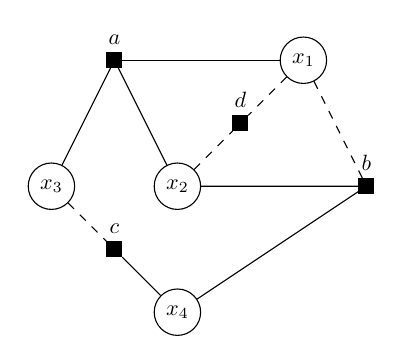
\begin{tikzpicture}[scale=0.8,transform shape]
   	\node[shape=circle,draw=black] (x1) at (3,0) {$x_1$};
    \node[shape=circle,draw=black] (x2) at (1,-2) {$x_2$};
    \node[shape=circle,draw=black] (x3) at (-1,-2) {$x_3$};
    \node[shape=circle,draw=black] (x4) at (1,-4) {$x_4$};
    
    \node[rectangle,draw=black, label = {$a$}, fill] (a) at (0,0) {};
     \node[rectangle,draw=black, label = {$d$}, fill] (d) at (2,-1) {};
     \node[rectangle,draw=black, label = {$b$}, fill] (b) at (4,-2) {};
     \node[rectangle,draw=black, label = {$c$}, fill] (c) at (0,-3) {};
     
 
    \path [-] (x1) edge node[left] {} (a);
    \path [-] (x2) edge node[left] {} (a);
    \path [-] (x3) edge node[left] {} (a);
    
    \path [dashed] (x1) edge node[left] {} (d);
    \path [dashed] (x2) edge node[left] {} (d);
    
    \path [-] (x2) edge node[left] {} (b);
    \path [dashed] (x1) edge node[left] {} (b);
    \path [-] (x4) edge node[left] {} (b);
    
    \path [-] (x4) edge node[left] {} (c);
    \path [dashed] (x3) edge node[left] {} (c);
\end{tikzpicture}
\end{figure}
\end{column}
\end{columns}
\end{minipage}	
\end{frame}


\begin{frame}
	\frametitle{Message Passing}
	Message Passing Algorithms on factor graphs
	\begin{itemize}
		\item Nodes communicate through messages
		\item Messages are passed over the graph's edges
		\item Two types of messages
			\begin{itemize}
				\item $\mu_{i \rightarrow a}$ sent from factor $a$ to variable $i$
				\item $\mu_{a \rightarrow i}$ sent from variable $i$ to factor $a$
			\end{itemize}	
	\end{itemize}
	\begin{figure}
\centering

\begin{tikzpicture}[scale=0.8,transform shape, >=stealth]
   	\node[shape=circle,draw=black] (i) at (3,0) {$i$};
   \tikzset{myptr/.style={decoration={markings,mark=at position 1 with %
    {\arrow[scale=3,>=stealth]{>}}},postaction={decorate}}}
    
    \node[rectangle,draw=black, label = {$a$}, fill] (a) at (0,0) {};
    
 	\only<1>{    \path [-] (i) edge node[left] {} (a);}

    \only<2> {\path [->] (i) edge node[left, above] {$\mu_{i \rightarrow a}$} (a);}
    \only<3>{\path [<-] (i) edge node[left, above] {$\mu_{a \rightarrow i}$} (a);}
    
    %\path [dashed] (x3) edge node[left] {} (c);
\end{tikzpicture}
\end{figure}
		
\end{frame}

\begin{frame}
	\frametitle{Message Passing}
	Message Passing Algorithms on factor graphs
	\begin{itemize}
		\item Message $\mu_{a \rightarrow i}$ determined by incoming messages $\mu_{j \rightarrow a}$ from neighbours $j \neq i$
		\item Computation Rule depends on application
			
	\end{itemize}
\begin{figure}
\centering

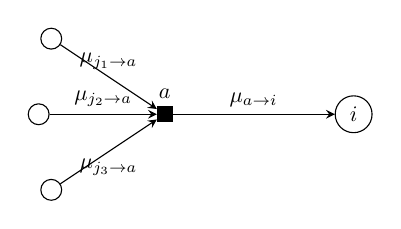
\begin{tikzpicture}[scale=0.8,transform shape, >=stealth]
   	\node[shape=circle,draw=black] (i) at (3,0) {$i$};
   \tikzset{myptr/.style={decoration={markings,mark=at position 1 with %
    {\arrow[scale=3,>=stealth]{>}}},postaction={decorate}}}
    
    \node[rectangle,draw=black, label = {$a$}, fill] (a) at (0,0) {};
    
	\node[shape=circle,draw=black] (j1) at (-1.8,1.2) {};    
	\node[shape=circle,draw=black] (j2) at (-2,0) {};    
	\node[shape=circle,draw=black] (j3) at (-1.8,-1.2) {};    

    
 	\path [->] (a) edge node[left, above] {$\mu_{a \rightarrow i}$} (i);
 	
 	\path [->] (j1) edge node[left, above] {$\mu_{j_1 \rightarrow a}$} (a);
 	\path [->] (j2) edge node[left, above] {$\mu_{j_2 \rightarrow a}$} (a);
 	\path [->] (j3) edge node[right, below] {$\mu_{j_3 \rightarrow a}$} (a);

   
    
    %\path [dashed] (x3) edge node[left] {} (c);
\end{tikzpicture}
\end{figure}
		
\end{frame}



\begin{frame}
	\frametitle{Message Passing}
	Message Passing Algorithms on trees
	\begin{itemize}
		\item Messages generated bottom up
		\item Leaves start sending messages
		\item Messages are propagated forward in the tree
		\item Does \textbf{not} work on graphs with cycles
	\end{itemize}
\end{frame}

\begin{frame}
\frametitle{Example}
\begin{figure}[h]
\centering

\begin{tikzpicture}[scale=0.8,transform shape, decoration={
       markings,
       mark=at position 1 with {\arrow[scale=2,black]{latex}};
     }]
   	\node[rectangle,draw=black, label = {$a$}, fill] (i) at (3,0) {$a$};
    \node[shape=circle,draw=black] (a) at (5,0) {$i$};
   
  \node[shape=circle,draw=black] (b1) at (0,2) {$j_1$};
  \node[shape=circle,draw=black] (b2) at (0,0) {$j_2$};
  \node[shape=circle,draw=black] (b3) at (0,-2) {$j_3$};

	\node[rectangle,draw=black, label = {$b_1$}, fill] (j1) at (-3,3) {};
	\node[rectangle,draw=black, label = {$b_2$}, fill] (j2) at (-3,1) {};
	\node[rectangle,draw=black, label = {$b_3$}, fill] (j3) at (-3,-1) {};
	\node[rectangle,draw=black, label = {$b_4$}, fill] (j4) at (-3,-3) {};

\tikzset{myptr/.style={decoration={markings,mark=at position 1 with %
    {\arrow[scale=1,>=stealth]{>}}},postaction={decorate}}}

    \only<1-1>{\draw[-, >= stealth] (b1) edge [right] node {} (j1);}
	\only<2-17>{\draw[-] (j1) edge [right, myptr] node[] {} (b1);}
	\only<14-17>{\draw[-] (b1) edge [right, myptr] node {} (j1);}
	
	\only<1-2>{\draw[-] (b2) edge [right] node {} (j2);}
	\only<3-17>{\draw[-] (j2) edge [right, myptr] node {} (b2);}
	\only<15-17>{\draw[-] (b2) edge [right, myptr] node {} (j2);}
	
	\only<1-3>{\draw[-] (b2) edge [right] node {} (j3);}
	\only<4-17>{\draw[-] (j3) edge [right, myptr] node {} (b2);}
	\only<16-17>{\draw[-] (b2) edge [right, myptr] node {} (j3);}
	
	\only<1-4>{\draw[-, >= stealth] (b3) edge [right] node {} (j4);}
	\only<5-17>{\draw[-] (j4) edge [right, myptr] node {} (b3);}
	\only<17-17>{\draw[-] (b3) edge [right, myptr] node {} (j4);}
	
	\only<1-5>{\draw[-] (i) edge [right] node {} (a);}
	\only<6-17>{\draw[-] (a) edge [right, myptr] node {} (i);}
	\only<12-17>{\draw[-] (i) edge [right, myptr] node {} (a);}
	
	\only<1-6>{\draw[-] (b1) edge [right] node {} (i);}
	\only<7-17>{\draw[-] (b1) edge [right, myptr] node {} (i);}
	\only<13-17>{\draw[-] (i) edge [right, myptr] node {} (b1);}
	
	\only<1-7>{\draw[-, >= stealth] (b2) edge [right] node {} (i);}
	\only<8-17>{\draw[-] (b2) edge [right, myptr] node {} (i);}
	\only<10-17>{\draw[-] (i) edge [right, myptr] node {} (b2);}
	
	\only<1-8>{\draw[-] (b3) edge [right] node {} (i);}
	\only<9-17>{\draw[-] (b3) edge [right, myptr] node {} (i);}
	\only<11-17>{\draw[-] (i) edge [right, myptr] node {} (b3);}
	
\end{tikzpicture}
%\caption{Subgraph of a factor tree with all messages required for computing $m_{a \rightarrow i}$}
\end{figure}
\end{frame}

\begin{frame}
	\frametitle{Message Passing}
	\begin{itemize}
		\item In general graphs: \emph{Loopy} Message Passing
		\item Messages initialized with random values
		\item Each node repeatedly updates its outgoing messages based on the incoming ones
		\item Goal: \emph{Convergence}
		\item Scheduling important
	\end{itemize}

		
\end{frame}

\begin{frame}[containsverbatim]
	\frametitle{Message Passing}
	Generic Message Passing Algorithm
	\begin{lstlisting}[mathescape = true, gobble=15, basicstyle=\ttfamily]
		1. Randomly initialize all warnings $\mu_{i \rightarrow a}, \mu_{a \rightarrow i}$
		2. For $t = 0$ to $t_{max}$
		  2.1 Apply the update rule to all edges
		      in random order
		  2.2 If no message has changed goto 3
		3. If $t = t_{max}$ return UNGONVERGED
		   Else      return the converged messages
	\end{lstlisting}
\end{frame}

\begin{frame}
	\frametitle{Message Passing}
	\begin{itemize}
		\item Loopy Message Passing converges on trees
		\item On cyclic graphs
			\begin{itemize}
				\item no guarantee of convergence
				\item no guarantee of correctness
			\end{itemize}
		\item Can be used as heuristics
		\item In practice often correct
			\end{itemize}
\end{frame}
